\subsection{Identificación dependencias}
\par Solo analizo los bucles internos, porque la vectorización consiste en ejecutar en paralelo las operaciones matemáticas realizadas en 
los bucles internos de aplicaciones de código científico.
\par Hay varias estrategias para usar código vectorial en los programas, en este caso dejo que el compilador 
vectorice automáticamente.


\subsubsection{\textbf{1ºBucle:}}
\par El primer bucle es \texttt{while(difference / (state.height * state.width) > tolerance)}. Se podría paralelizar creando una rama master y añadiendo un pragma de tipo
\texttt{task} que comparte la variable \texttt{iterations} antes del \texttt{if(verbose)} porque la ejecución de la siguiente iteración no depende de esto.
Además, dentro de esta \texttt{task} se necesita un pragma \texttt{atomic}, porque solo un hilo puede modificar a la vez esa variable global. Esta
implementación, mostrada en el código siguiente, no ayuda mucho en el rendimiento de la aplicación y la mejora es despreciable e incluso en 
algunos casos es peor como se indica en todas las tablas y gráficas.
%%% TABLA DE TIEMPOS E IMÁGENES %%%
\begin{figure}[H]
    \centering
    \begin{subfigure}{0.4\textwidth}
        \begin{adjustbox}{width=\textwidth} 
        \begin{tabular}{|c|c|c|c|c|}
            \hline
            \rowcolor{azul} \multicolumn{2}{|c|}{}&\multicolumn{3}{c|}{\textbf{Compiler}} \\ \hline
            \rowcolor{azul} \multicolumn{2}{|c|}{}&\texttt{clang}&\texttt{gcc}&\texttt{icc}\\ \hline
            \rowcolor{azul} \textbf{Testing size} & \textbf{Threads}&\multicolumn{3}{c|}{\textbf{Average time (s)}} \\ \hline
            \multirow{8}{1cm}{\textbf{01-small}} & 1 & \(1.58\pm{0.03}\) & \(0.32\pm{0.01}\) & \(1.00\pm{0.01}\) \\ \cline{2-5}
            & 2 & \(1.58\pm{0.03}\) & \(0.32\pm{0.01}\) & \(1.02\pm{0.01}\) \\ \cline{2-5}
            & 3 & \(1.60\pm{0.03}\) & \(0.33\pm{0.01}\) & \(1.02\pm{0.01}\) \\ \cline{2-5}
            & 4 & \(1.62\pm{0.01}\) & \(0.33\pm{0.01}\) & \(1.08\pm{0.04}\) \\ \cline{2-5}
            & 5 & \(1.62\pm{0.01}\) & \(0.33\pm{0.01}\) & \(1.05\pm{0.01}\) \\ \cline{2-5}
            & 6 & \(1.72\pm{0.01}\) & \(0.46\pm{0.01}\) & \(1.41\pm{0.35}\) \\ \cline{2-5}
            & 7 & \(1.99\pm{0.01}\) & \(0.47\pm{0.01}\) & \(1.44\pm{0.32}\) \\ \cline{2-5}
            & 8 & \(1.85\pm{0.01}\) & \(0.47\pm{0.02}\) & \(1.77\pm{0.02}\) \\ \hline
        \end{tabular}
        \end{adjustbox}
    \end{subfigure}
    \hfill
    \begin{subfigure}{0.5\textwidth}
        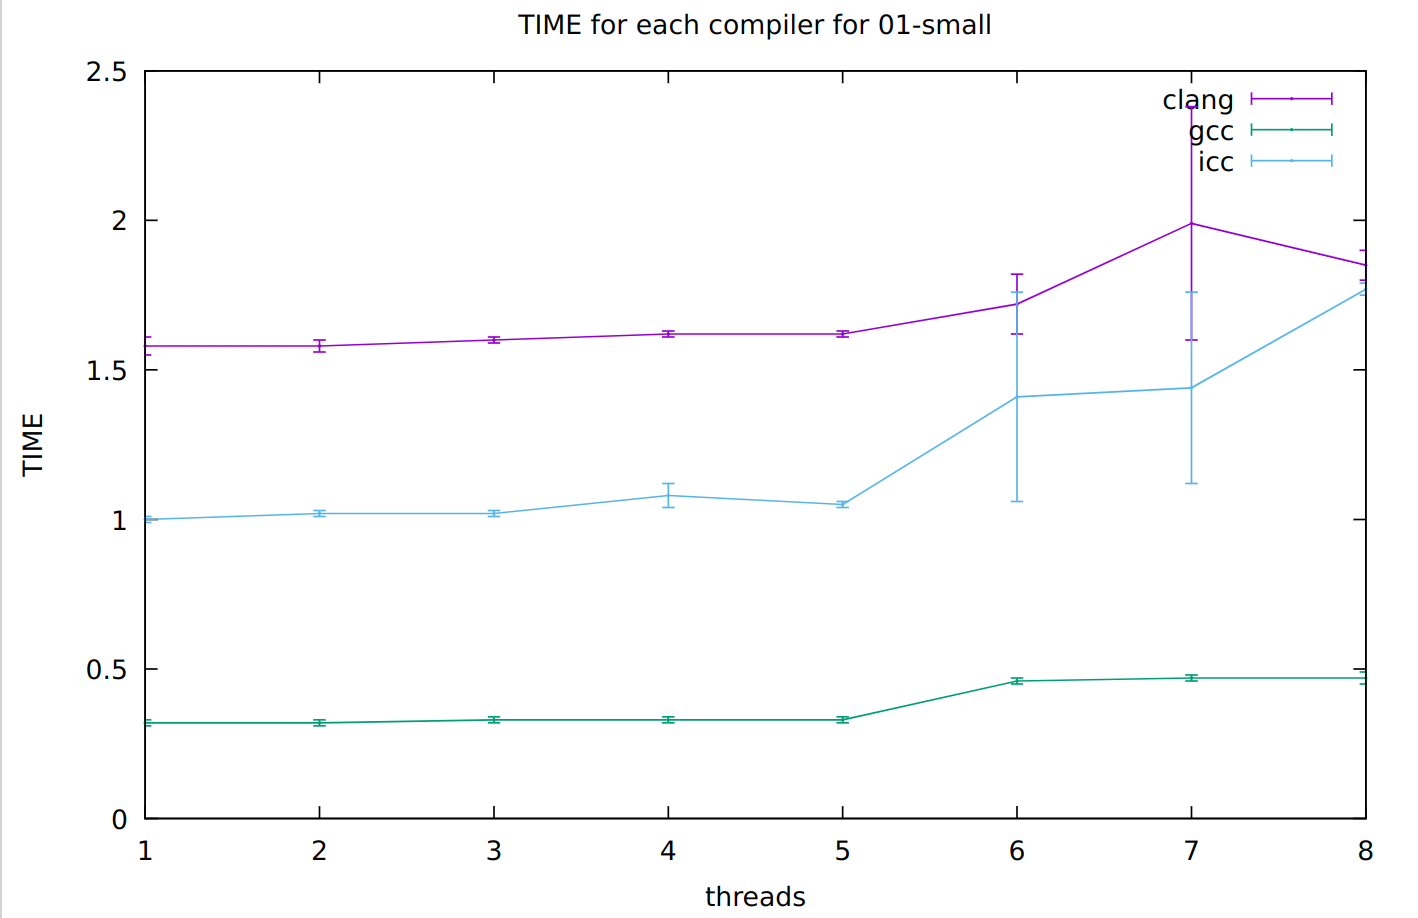
\includegraphics[width=\textwidth]{bucle1=01-small}
    \end{subfigure}
    \caption{\underline{1º Bucle, tamaño pequeño}: Tiempos de ejecución vs nº de hilos}
    \label{fig:bucle1=01-small}
\end{figure}
\newpage

\subsubsection{\textbf{heat.cpp}}
\begin{listing}[firstnumber=20]
    @@ -21,28 +21,36 @@
    void solve(Matrix<double>& state, double tolerance, int& iterations, double& last_difference) {
    Matrix<double> next_state = state;
    iterations = 0;
    double difference;
  + #pragma omp parallel
  + {
  + #pragma omp master
    do {
        difference = 0;
        for (size_t i = 1; i < state.height - 1; ++i) {
            for (size_t j = 1; j < state.width - 1; ++j) {
                next_state[i][j] = (state[i][j]
                                + state[i + 1][j]  
                                + state[i - 1][j]  
                                + state[i][j + 1]  
                                + state[i][j - 1]) / 5;
                difference = difference 
                             + abs(next_state[i][j]-state[i][j]);
            }
        }

        state.swap_data(next_state);

  + #pragma omp task shared(iterations)
  + {    
        if (verbose) {
            cout << "Iteration " << iterations << ":" << endl;
            printf_matrix("%7.3f", state);
            cout << "Difference: " << difference << endl;
        }
  + #pragma omp atomic
        ++iterations;
  + }
    } while (difference / (state.height * state.width) > tolerance);
    last_difference = difference / (state.height * state.width);
  + }
    }
\end{listing}


%%% TABLA DE TIEMPOS E IMÁGENES %%%
\begin{figure}[H]
    \centering
    \begin{subfigure}{0.4\textwidth}
        \begin{adjustbox}{width=\textwidth} 
        \begin{tabular}{|c|c|c|c|c|}
            \hline
            \rowcolor{azul} \multicolumn{2}{|c|}{}&\multicolumn{3}{c|}{\textbf{Compiler}} \\ \hline
            \rowcolor{azul} \multicolumn{2}{|c|}{}&\texttt{clang}&\texttt{gcc}&\texttt{icc}\\ \hline
            \rowcolor{azul} \textbf{Testing size} & \textbf{Threads}&\multicolumn{3}{c|}{\textbf{Average time (s)}} \\ \hline
            \multirow{8}{2.5cm}{\textbf{02-medium}} & 1 & \(4.83\pm{0.42}\) & \(0.89\pm{0.04}\) & \(2.88\pm{0.04}\) \\ \cline{2-5}
            & 2 & \(4.73\pm{0.24}\) & \(0.91\pm{0.04}\) & \(2.94\pm{0.04}\) \\ \cline{2-5}
            & 3 & \(4.57\pm{0.07}\) & \(0.90\pm{0.03}\) & \(3.22\pm{0.22}\) \\ \cline{2-5}
            & 4 & \(5.19\pm{0.57}\) & \(0.93\pm{0.04}\) & \(3.19\pm{0.21}\) \\ \cline{2-5}
            & 5 & \(4.63\pm{0.04}\) & \(1.28\pm{0.03}\) & \(3.16\pm{0.15}\) \\ \cline{2-5}
            & 6 & \(4.63\pm{0.03}\) & \(1.27\pm{0.03}\) & \(4.20\pm{0.86}\) \\ \cline{2-5}
            & 7 & \(4.64\pm{0.03}\) & \(1.27\pm{0.03}\) & \(4.83\pm{0.24}\) \\ \cline{2-5}
            & 8 & \(5.41\pm{0.08}\) & \(1.20\pm{0.04}\) & \(5.17\pm{0.10}\) \\ \hline
        \end{tabular}
        \end{adjustbox}
    \end{subfigure}
    \hfill
    \begin{subfigure}{0.5\textwidth}
        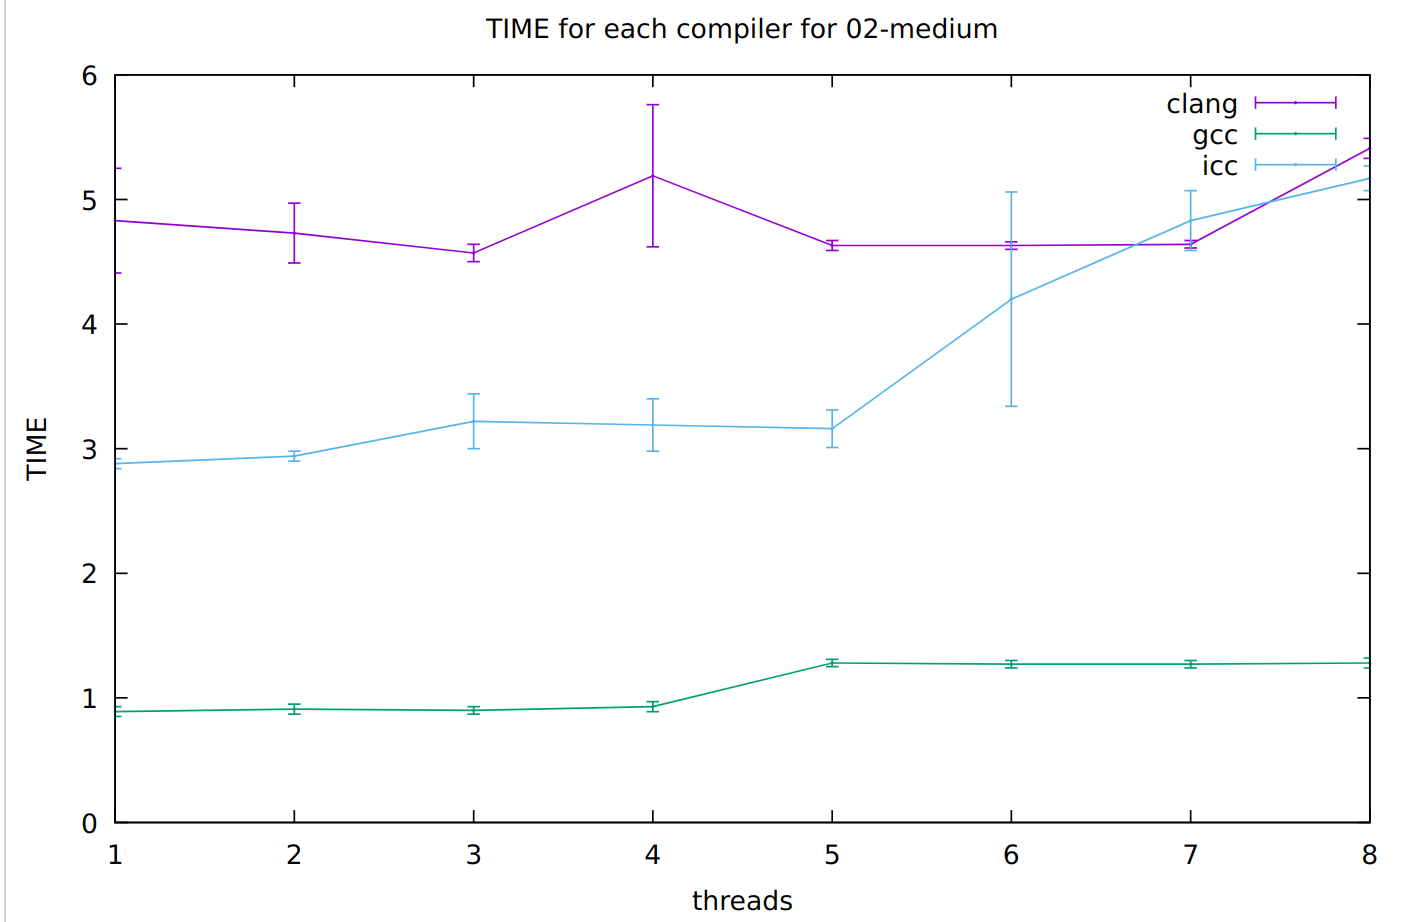
\includegraphics[width=\textwidth]{bucle1=02-medium}
    \end{subfigure}
    \caption{\underline{1º Bucle, tamaño mediano}: Tiempos de ejecución vs nº de hilos}
    \label{bucle1=02-medium}
\end{figure}

%%% TABLA DE TIEMPOS E IMÁGENES %%%
\begin{figure}[H]
    \centering
    \begin{subfigure}{0.4\textwidth}
        \begin{adjustbox}{width=\textwidth} 
        \begin{tabular}{|c|c|c|c|c|}
            \hline
            \rowcolor{azul} \multicolumn{2}{|c|}{}&\multicolumn{3}{c|}{\textbf{Compiler}} \\ \hline
            \rowcolor{azul} \multicolumn{2}{|c|}{}&\texttt{clang}&\texttt{gcc}&\texttt{icc}\\ \hline
            \rowcolor{azul} \textbf{Testing size} & \textbf{Threads}&\multicolumn{3}{c|}{\textbf{Average time (s)}} \\ \hline
            \multirow{8}{1cm}{\textbf{03-large}} & 1 & \(7.58\pm{0.01}\) & \(1.54\pm{0.11}\) & \(4.97\pm{0.13}\) \\ \cline{2-5}
            & 2 & \(7.69\pm{0.05}\) & \(1.55\pm{0.07}\) & \(5.11\pm{0.16}\) \\ \cline{2-5}
            & 3 & \(7.83\pm{0.01}\) & \(1.56\pm{0.08}\) & \(5.20\pm{0.21}\) \\ \cline{2-5}
            & 4 & \(7.87\pm{0.06}\) & \(1.61\pm{0.09}\) & \(5.23\pm{0.16}\) \\ \cline{2-5}
            & 5 & \(7.90\pm{0.03}\) & \(2.19\pm{0.05}\) & \(5.23\pm{0.18}\) \\ \cline{2-5}
            & 6 & \(7.87\pm{0.05}\) & \(2.17\pm{0.05}\) & \(5.20\pm{0.14}\) \\ \cline{2-5}
            & 7 & \(8.86\pm{0.01}\) & \(2.16\pm{0.06}\) & \(8.78\pm{0.18}\) \\ \cline{2-5}
            & 8 & \(8.85\pm{0.03}\) & \(2.15\pm{0.03}\) & \(8.76\pm{0.15}\) \\ \hline
        \end{tabular}
        \end{adjustbox}
    \end{subfigure}
    \hfill
    \begin{subfigure}{0.5\textwidth}
        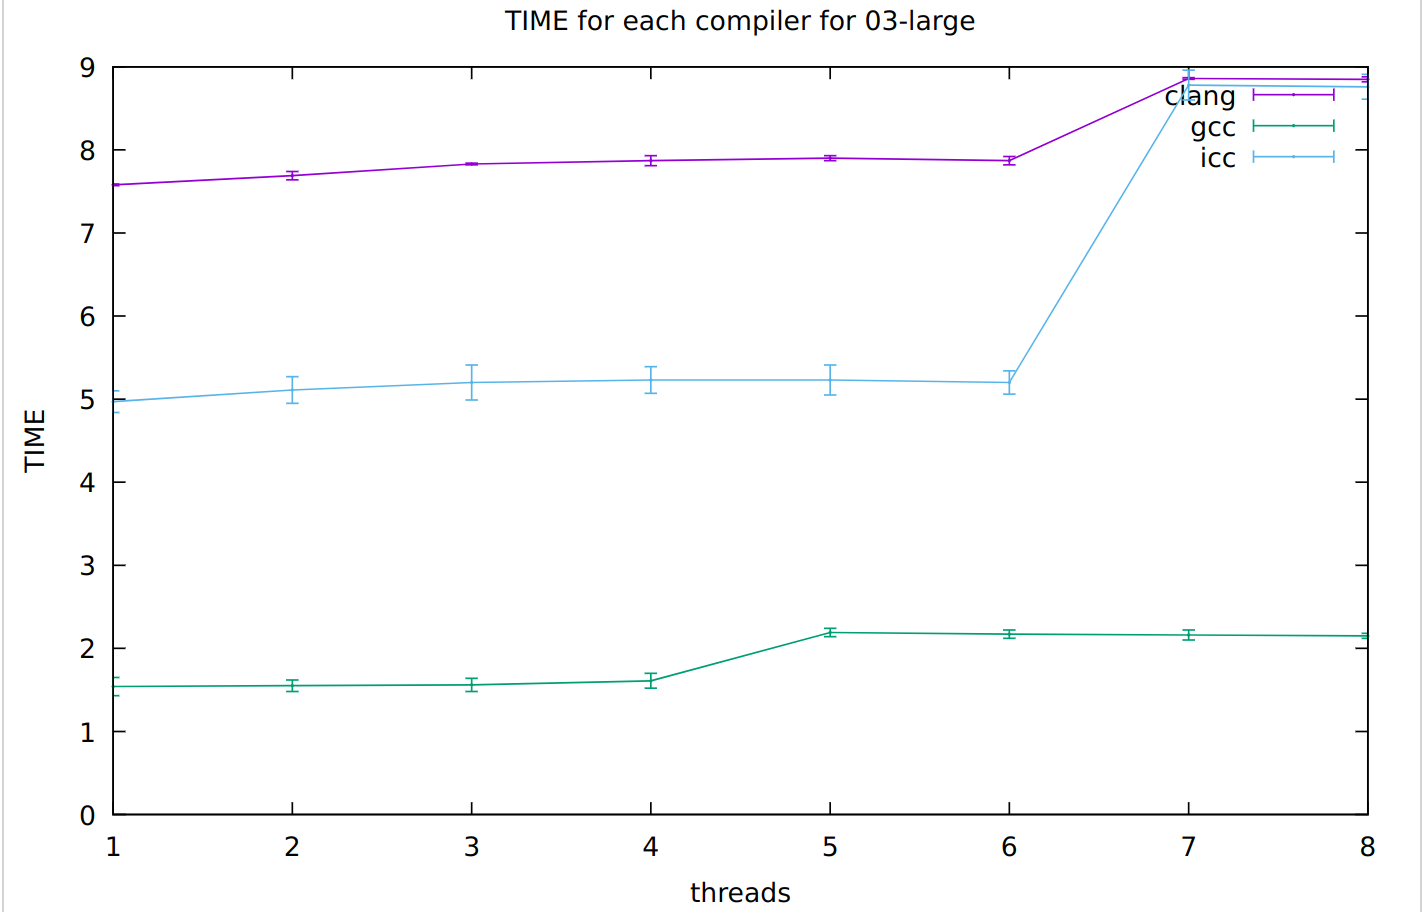
\includegraphics[width=\textwidth]{bucle1=03-large}
    \end{subfigure}
    \caption{\underline{1º Bucle, tamaño largo}: Tiempos de ejecución vs nº de hilos}
    \label{bucle1=03-large}
\end{figure}

\subsubsection{\textbf{2ºBucle:}}

\par El segundo es el bucle exterior \texttt{for (size\_t i = 1; i < state.height - 1; ++i)}, es el mejor candidato para paralelizar, hay que añadir un
pragma \texttt{\#pragma omp parallel for reduction (max:difference)} para que ejecute las instrucciones en paralelo pero tenga en cuenta la
instrucción max que no deben de ejecutarla dos hilos a la vez.

%%% TABLA DE TIEMPOS E IMÁGENES %%%
\begin{figure}[H]
    \centering
    \begin{subfigure}{0.4\textwidth}
        \begin{adjustbox}{width=\textwidth} 
        \begin{tabular}{|c|c|c|c|c|}
            \hline
            \rowcolor{azul} \multicolumn{2}{|c|}{}&\multicolumn{3}{c|}{\textbf{Compiler}} \\ \hline
            \rowcolor{azul} \multicolumn{2}{|c|}{}&\texttt{clang}&\texttt{gcc}&\texttt{icc}\\ \hline
            \rowcolor{azul} \textbf{Testing size} & \textbf{Threads}&\multicolumn{3}{c|}{\textbf{Average time (s)}} \\ \hline
            \multirow{8}{1cm}{\textbf{01-small}} & 1 & \(1.53\pm{0.00}\) & \(0.36\pm{0.00}\) & \(1.01\pm{0.01}\) \\ \cline{2-5}
            & 2 & \(0.81\pm{0.02}\) & \(0.18\pm{0.01}\) & \(0.53\pm{0.01}\) \\ \cline{2-5}
            & 3 & \(0.54\pm{0.00}\) & \(0.13\pm{0.01}\) & \(0.37\pm{0.00}\) \\ \cline{2-5}
            & 4 & \(0.42\pm{0.00}\) & \(0.12\pm{0.03}\) & \(0.34\pm{0.05}\) \\ \cline{2-5}
            & 5 & \(0.41\pm{0.01}\) & \(0.14\pm{0.01}\) & \(0.45\pm{0.01}\) \\ \cline{2-5}
            & 6 & \(0.35\pm{0.01}\) & \(0.13\pm{0.02}\) & \(0.40\pm{0.03}\) \\ \cline{2-5}
            & 7 & \(0.31\pm{0.01}\) & \(0.11\pm{0.00}\) & \(0.33\pm{0.01}\) \\ \cline{2-5}
            & 8 & \(0.29\pm{0.01}\) & \(0.11\pm{0.00}\) & \(0.33\pm{0.02}\) \\ \hline
        \end{tabular}
        \end{adjustbox}
    \end{subfigure}
    \hfill
    \begin{subfigure}{0.5\textwidth}
        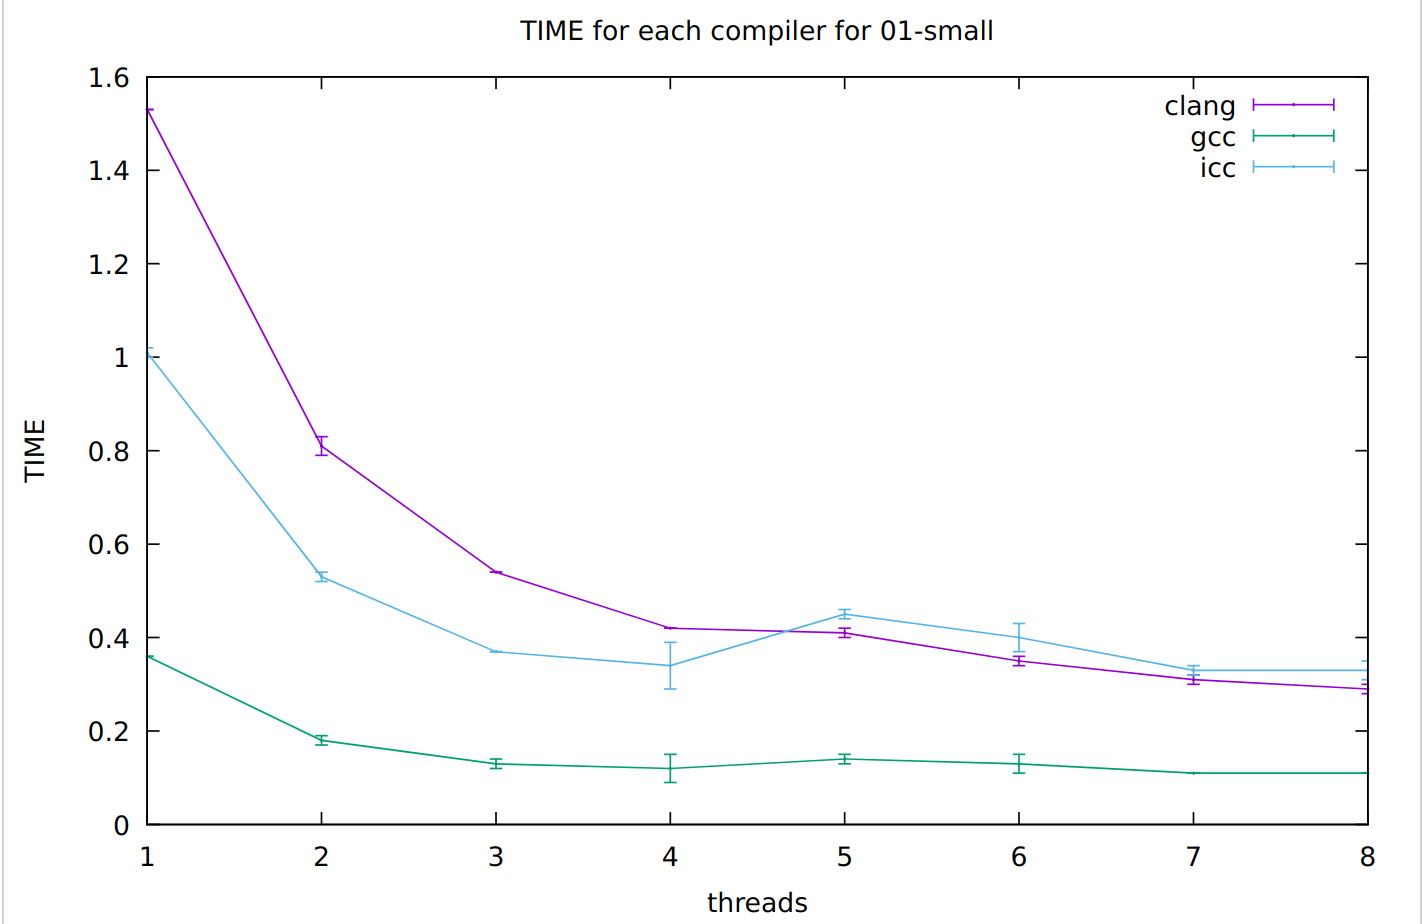
\includegraphics[width=\textwidth]{bucle2=01-small}
    \end{subfigure}
    \caption{\underline{Tamaño pequeño}: Tiempos de ejecución vs nº de hilos}
    \label{fig:bucle2=01-small}
\end{figure}

%%% TABLA DE TIEMPOS E IMÁGENES %%%
\begin{figure}[H]
    \centering
    \begin{subfigure}{0.4\textwidth}
        \begin{adjustbox}{width=\textwidth} 
        \begin{tabular}{|c|c|c|c|c|}
            \hline
            \rowcolor{azul} \multicolumn{2}{|c|}{}&\multicolumn{3}{c|}{\textbf{Compiler}} \\ \hline
            \rowcolor{azul} \multicolumn{2}{|c|}{}&\texttt{clang}&\texttt{gcc}&\texttt{icc}\\ \hline
            \rowcolor{azul} \textbf{Testing size} & \textbf{Threads}&\multicolumn{3}{c|}{\textbf{Average time (s)}} \\ \hline
            \multirow{8}{2.5cm}{\textbf{02-medium}} & 1 & \(4.45\pm{0.03}\) & \(0.89\pm{0.03}\) & \(2.90\pm{0.03}\) \\ \cline{2-5}
            & 2 & \(2.31\pm{0.05}\) & \(0.47\pm{0.02}\) & \(3.37\pm{0.06}\) \\ \cline{2-5}
            & 3 & \(1.52\pm{0.00}\) & \(0.33\pm{0.02}\) & \(2.93\pm{0.05}\) \\ \cline{2-5}
            & 4 & \(1.20\pm{0.03}\) & \(0.30\pm{0.06}\) & \(2.97\pm{0.03}\) \\ \cline{2-5}
            & 5 & \(1.16\pm{0.04}\) & \(0.37\pm{0.02}\) & \(2.96\pm{0.02}\) \\ \cline{2-5}
            & 6 & \(0.97\pm{0.03}\) & \(0.31\pm{0.01}\) & \(2.96\pm{0.07}\) \\ \cline{2-5}
            & 7 & \(0.87\pm{0.05}\) & \(0.27\pm{0.01}\) & \(2.93\pm{0.02}\) \\ \cline{2-5}
            & 8 & \(0.77\pm{0.03}\) & \(0.25\pm{0.01}\) & \(2.92\pm{0.01}\) \\ \hline
        \end{tabular}
        \end{adjustbox}
    \end{subfigure}
    \hfill
    \begin{subfigure}{0.5\textwidth}
        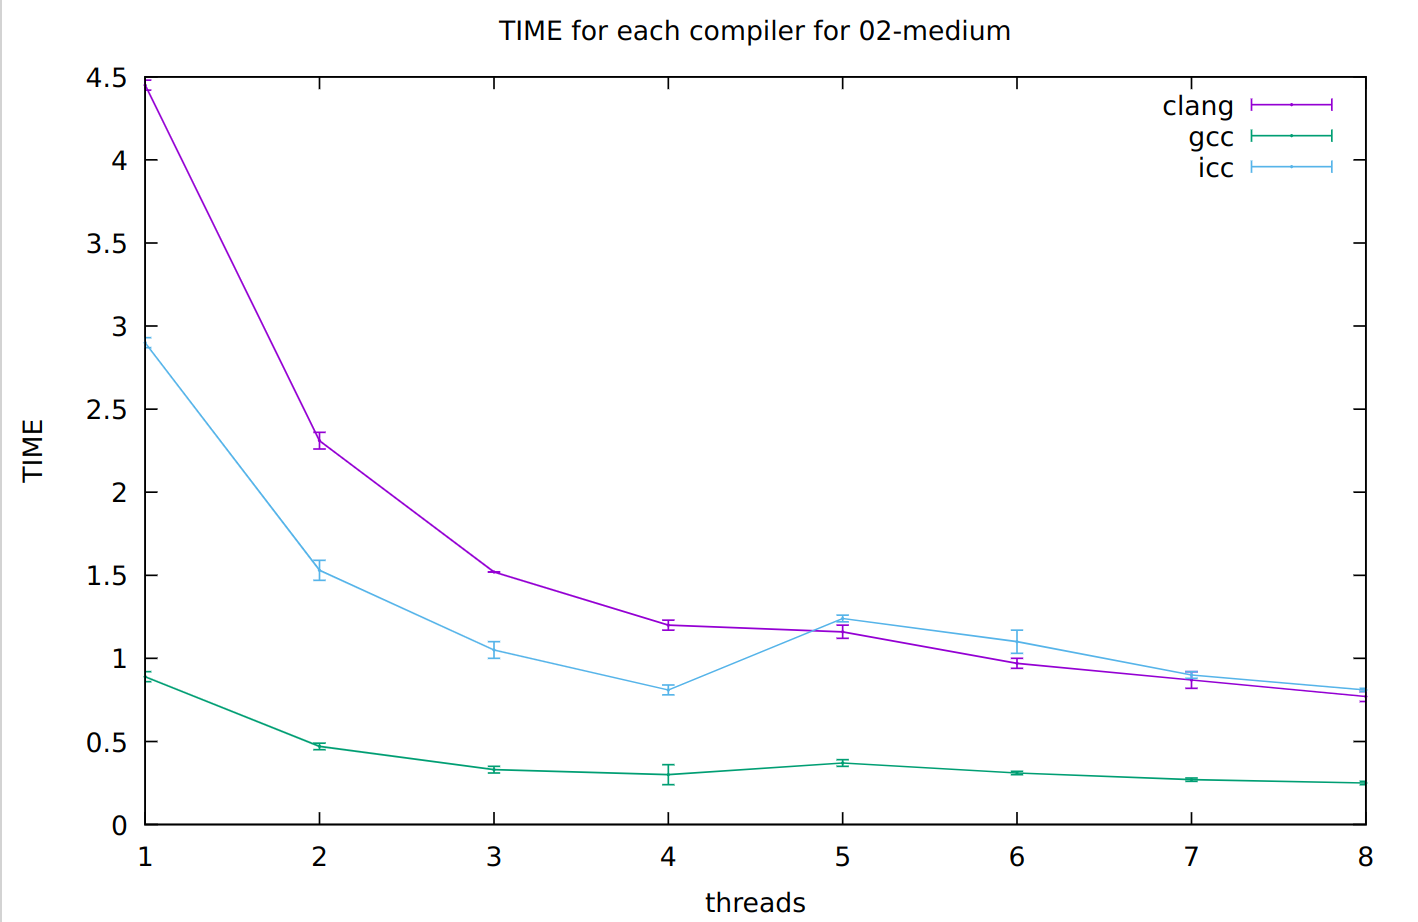
\includegraphics[width=\textwidth]{bucle2=02-medium}
    \end{subfigure}
    \caption{\underline{Tamaño mediano}: Tiempos de ejecución vs nº de hilos}
    \label{bucle2=02-medium}
\end{figure}

%%% TABLA DE TIEMPOS E IMÁGENES %%%
\begin{figure}[H]
    \centering
    \begin{subfigure}{0.4\textwidth}
        \begin{adjustbox}{width=\textwidth} 
        \begin{tabular}{|c|c|c|c|c|}
            \hline
            \rowcolor{azul} \multicolumn{2}{|c|}{}&\multicolumn{3}{c|}{\textbf{Compiler}} \\ \hline
            \rowcolor{azul} \multicolumn{2}{|c|}{}&\texttt{clang}&\texttt{gcc}&\texttt{icc}\\ \hline
            \rowcolor{azul} \textbf{Testing size} & \textbf{Threads}&\multicolumn{3}{c|}{\textbf{Average time (s)}} \\ \hline
            \multirow{8}{1cm}{\textbf{03-large}} & 1 & \(7.62\pm{0.15}\) & \(1.56\pm{0.07}\) & \(5.00\pm{0.12}\) \\ \cline{2-5}
            & 2 & \(3.93\pm{0.05}\) & \(0.80\pm{0.04}\) & \(2.63\pm{0.11}\) \\ \cline{2-5}
            & 3 & \(2.65\pm{0.02}\) & \(0.55\pm{0.04}\) & \(1.85\pm{0.15}\) \\ \cline{2-5}
            & 4 & \(2.02\pm{0.02}\) & \(0.42\pm{0.02}\) & \(1.37\pm{0.05}\) \\ \cline{2-5}
            & 5 & \(1.97\pm{0.12}\) & \(0.60\pm{0.03}\) & \(2.10\pm{0.02}\) \\ \cline{2-5}
            & 6 & \(1.67\pm{0.09}\) & \(0.51\pm{0.02}\) & \(1.78\pm{0.05}\) \\ \cline{2-5}
            & 7 & \(1.43\pm{0.07}\) & \(0.47\pm{0.04}\) & \(1.51\pm{0.02}\) \\ \cline{2-5}
            & 8 & \(1.28\pm{0.06}\) & \(0.41\pm{0.02}\) & \(1.40\pm{0.05}\) \\ \hline
        \end{tabular}
        \end{adjustbox}
    \end{subfigure}
    \hfill
    \begin{subfigure}{0.5\textwidth}
        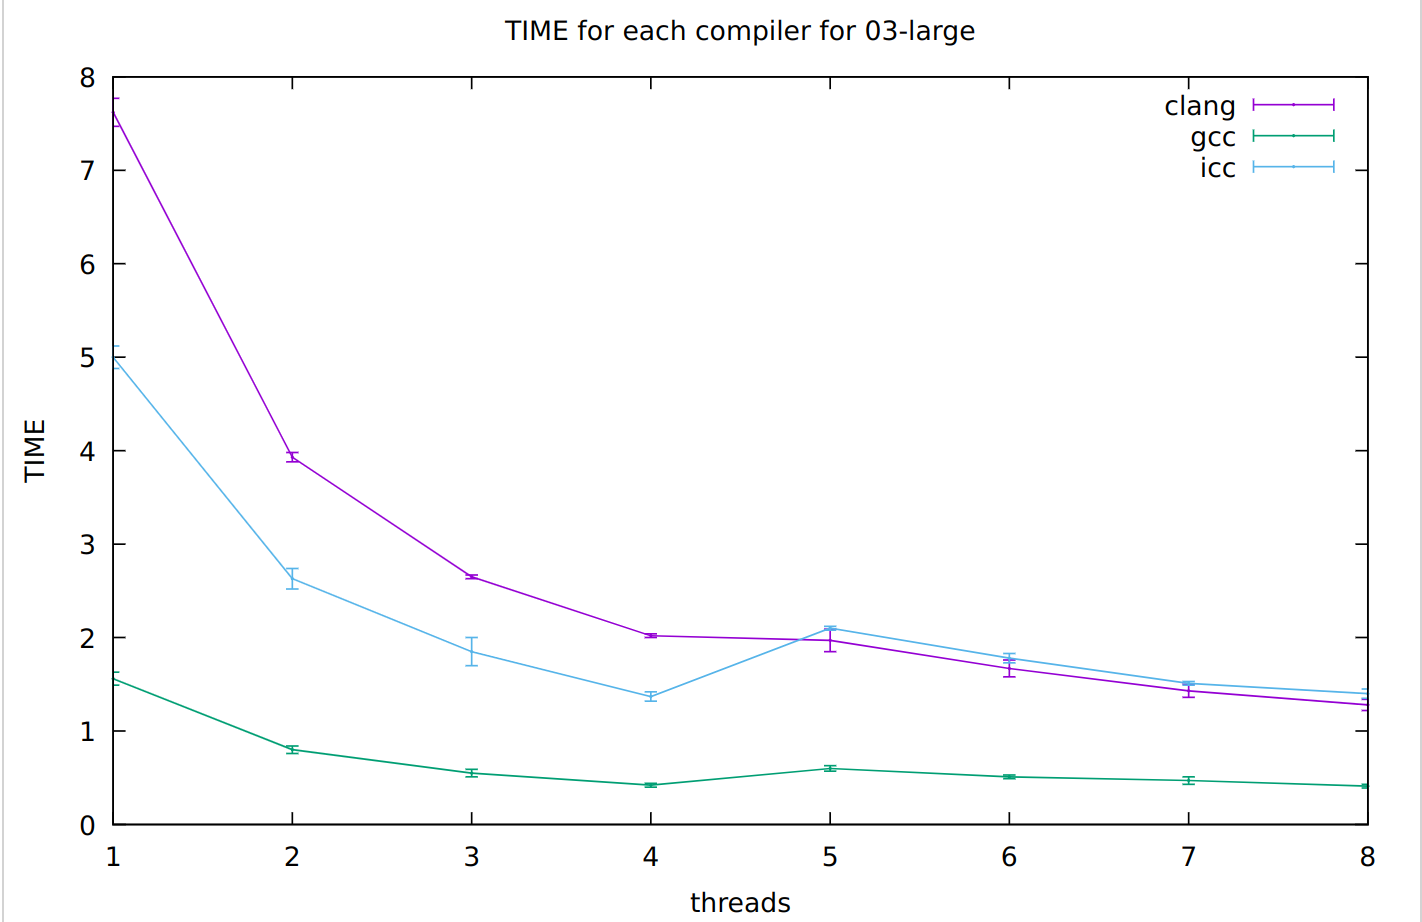
\includegraphics[width=\textwidth]{bucle2=03-large}
    \end{subfigure}
    \caption{\underline{Tamaño largo}: Tiempos de ejecución vs nº de hilos}
    \label{bucle2=03-large}
\end{figure}
\subsubsection{\textbf{3ºBucle:}}
\begin{listing}
    @@ -20,3 +20,4 @@
\end{listing}
\subsubsection{\textbf{4ºBucle:}}
\begin{listing}[firstnumber=31]
    @@ -32,3 +32,3 @@
    for (int i = 0; i < arrays_size; ++i) {
      C[i] = A[i] + 2 * B[i];
    }
\end{listing}
\par No hace falta analizar la ejecución desarrollada del bucle porque mirando el código se puede decir a simple vista que no hay
\textbf{ninguna dependencia} entre iteraciones, porque en cada iteración solo se necesita los valores que se leen y procesan en ella misma.
El compilador podrá vectorizar automáticamente este bucle sin ninguna modificación.
\subsubsection{\textbf{5ºBucle:}}
\begin{listing}[firstnumber=126]
    @@ -127,3 +127,3 @@
    LOOP BEGIN at loops.cpp(36,5)
        remark #15300: LOOP WAS VECTORIZED
    LOOP END
\end{listing}
\par Para saber como optimiza este bucle podemos ver el código ensamblador generado con el comando \texttt{\$ objdump -S loops | less}
en el que se puede ver como utiliza 8 registros para almacenar los totales parciales de ocho en ocho en cada iteración.

\begin{listing}[numbers=none, basicstyle=\scriptsize\ttfamily]
    400ee5: 0f ae f0                mfence
    400ee8: c5 7d 6f d1             vmovdqa %ymm1,%ymm10
    400eec: 33 c0                   xor %eax,%eax
    400eee: c4 41 25 57 db          vxorpd %ymm11,%ymm11,%ymm11
    400ef3: c5 7d 6f c9             vmovdqa %ymm1,%ymm9
    400ef7: c5 7d 6f c1             vmovdqa %ymm1,%ymm8
    400efb: c5 fd 6f f9             vmovdqa %ymm1,%ymm7
    400eff: c5 fd 6f f1             vmovdqa %ymm1,%ymm6
    400f03: c5 fd 28 e9             vmovapd %ymm1,%ymm5
    400f07: c5 fd 28 e1             vmovapd %ymm1,%ymm4
    400f0b: 0f 1f 44 00 00          nopl 0x0(%rax,%rax,1)
    400f10: c5 25 58 1c c5 60 61    vaddpd 0x1546160(,%rax,8),%ymm11,%ymm11
    400f17: 54 01
    400f19: c5 2d 58 14 c5 80 61    vaddpd 0x1546180(,%rax,8),%ymm10,%ymm10
    400f20: 54 01
    400f22: c5 35 58 0c c5 a0 61    vaddpd 0x15461a0(,%rax,8),%ymm9,%ymm9
    400f29: 54 01
    400f2b: c5 3d 58 04 c5 c0 61    vaddpd 0x15461c0(,%rax,8),%ymm8,%ymm8
    400f32: 54 01
    400f34: c5 c5 58 3c c5 e0 61    vaddpd 0x15461e0(,%rax,8),%ymm7,%ymm7
    400f3b: 54 01
    400f3d: c5 cd 58 34 c5 00 62    vaddpd 0x1546200(,%rax,8),%ymm6,%ymm6
    400f44: 54 01
    400f46: c5 d5 58 2c c5 20 62    vaddpd 0x1546220(,%rax,8),%ymm5,%ymm5
    400f4d: 54 01
    400f4f: c5 dd 58 24 c5 40 62    vaddpd 0x1546240(,%rax,8),%ymm4,%ymm4
    400f56: 54 01
    400f58: 48 83 c0 20             add $0x20,%rax
    400f5c: 48 3d 40 42 0f 00       cmp $0xf4240,%rax
    400f62: 72 ac                   jb 400f10 <main+0x200>
    400f64: c4 41 25 58 d2          vaddpd %ymm10,%ymm11,%ymm10
    400f69: fe c1                   inc %cl
    400f6b: c4 41 35 58 c0          vaddpd %ymm8,%ymm9,%ymm8
    400f70: c5 c5 58 f6             vaddpd %ymm6,%ymm7,%ymm6
    400f74: c5 d5 58 e4             vaddpd %ymm4,%ymm5,%ymm4
    400f78: c4 41 2d 58 c8          vaddpd %ymm8,%ymm10,%ymm9
    400f7d: c5 cd 58 ec             vaddpd %ymm4,%ymm6,%ymm5
    400f81: c5 b5 58 fd             vaddpd %ymm5,%ymm9,%ymm7
    400f85: c4 c3 7d 19 fb 01       vextractf128 $0x1,%ymm7,%xmm11
    400f8b: c4 41 41 58 e3          vaddpd %xmm11,%xmm7,%xmm12
    400f90: c4 41 19 15 ec          vunpckhpd %xmm12,%xmm12,%xmm13
    400f95: c4 41 1b 58 f5          vaddsd %xmm13,%xmm12,%xmm14
    400f9a: c5 8b 58 c0             vaddsd %xmm0,%xmm14,%xmm0
    400f9e: 80 f9 64                cmp $0x64,%cl
    400fa1: 0f 82 b2 fd ff ff       jb 400d59 <main+0x49>
\end{listing}
\par En \texttt{C} el código equivalente sería:
\begin{listing}[firstnumber=35]
    @@ -36,3 +36,11 @@
    + for (int i = 0; i < arrays_size; i+=8)
    + {
    +    ymm11 = ymm11 + c[i];
    +    ymm10 = ymm10 + c[i+1];
    +    ymm9 = ymm9 + c[i+2];
    +    ymm8 = ymm8 + c[i+3];
    +    ymm7 = ymm7 + c[i+4];
    +    ymm6 = ymm6 + c[i+5];
    +    ymm5 = ymm5 + c[i+6];
    +    ymm4 = ymm4 + c[i+7];
    + }
    + total = ymm11+ymm10+ymm9+ymm8+ymm7+ymm6+ymm5+ymm4+total;
\end{listing}